%This work is licensed under the Creative Commons License Attribution 4.0 International (CC-BY 4.0)
%https://creativecommons.org/licenses/by/4.0/legalcode
\documentclass[rgb]{standalone}
\usepackage{tkz-euclide}
\definecolor{myorange}{hsb}{0.0833, 1, 0.8}
\definecolor{mygreen}{hsb}{0.3333, 1, 0.8}
\definecolor{myblue}{hsb}{0.5833, 1, 0.8}
\definecolor{mymagenta}{hsb}{0.8333, 1, 0.8}
\begin{document}
	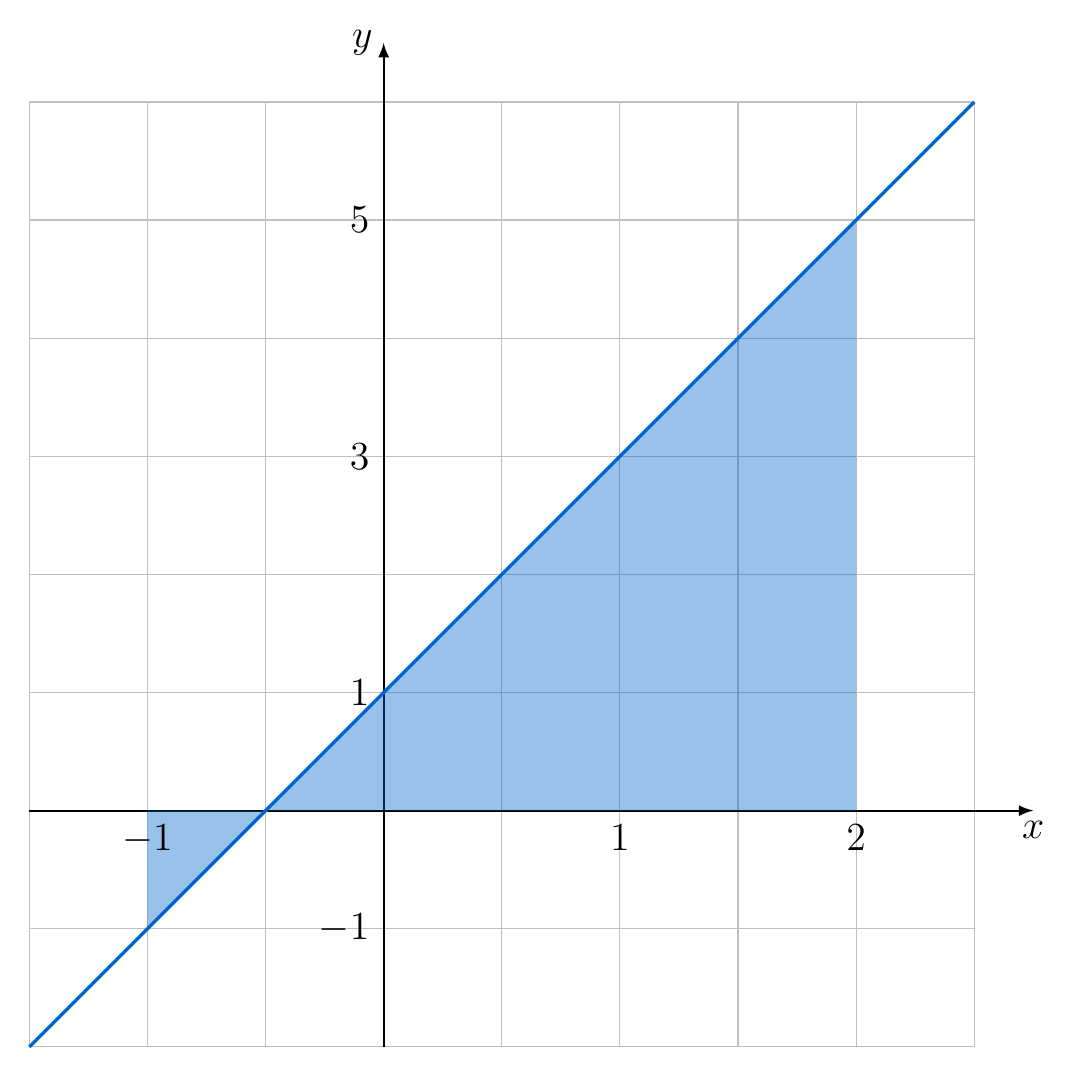
\begin{tikzpicture}[scale=1.5, font=\Large]
		% Coordinate system
		\tkzInit[xmin=-3,xmax=5,ymin=-2,ymax=6]
		\tkzGrid[color=lightgray]
		\tkzDrawX[thick]
		\tkzDrawY[thick]	
		\draw[fill,myblue, draw=none, fill opacity=0.4] (0,0) -- (4,0) -- (4,5) -- (-1,0);
		\draw[fill,myblue, draw=none, fill opacity=0.4] (-2,-1) -- (-2,0) -- (-1,0);
		\draw[very thick,myblue] (-3,-2) -- (5,6);		
		% Labely
		\node[below=0.5mm] at (-2,0){$-1$};
		\node[below=0.5mm] at (2,0){$1$};
		\node[below=0.5mm] at (4,0){$2$};
		\node[left=0.5mm] at (0,-1){$-1$};
		\node[left=0.5mm] at (0,1){$1$};
		\node[left=0.5mm] at (0,3){$3$};
		\node[left=0.5mm] at (0,5){$5$};
	\end{tikzpicture}	
\end{document}